\begin{figure}[t]
\centering
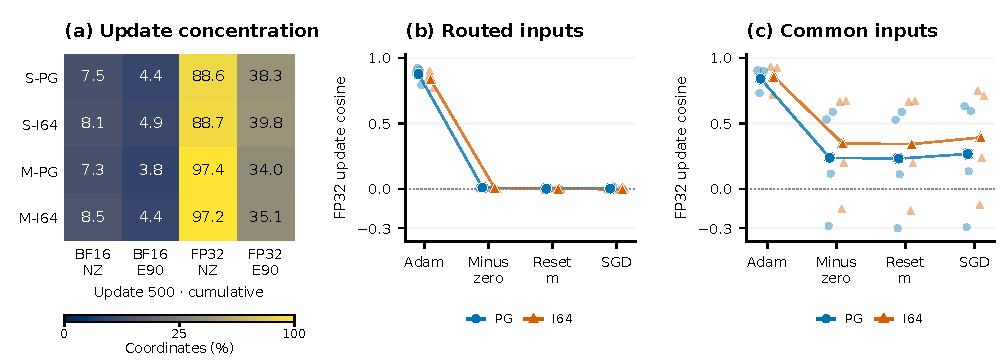
\includegraphics[width=\linewidth]{figures/nine_panel_20260914/section4_sparsity_overlap.pdf}
\caption{Parameter concentration and teacher-conditioned updates.
(a) Cumulative changes at update 500 for single-teacher (S) and joint (M) PG/I64 training, using DR. NZ is the nonzero coordinate fraction; E90 is the coordinate fraction carrying 90\% of squared change. Cells give percentages; color uses a square-root scale. S receives four times as many mathematics responses per update as M.
(b) At the common M-PG/500 student and optimizer state, FP32 top-1\% Jaccard versus signed update cosine. Small points average six teacher pairs within each bank; large points average four banks. Lines connect common-input (open) and routed-input (filled) conditions. SGD and reset-$m$ are individually norm-matched to saved-state Adam; circles denote PG and triangles I64.
(c) Teacher JS and $1-J$ on common inputs, with all six teacher pairs in all four banks. Colors and loss markers match (b); points share teachers and banks and are dependent. Updates use non-fused PyTorch steps on saved-state copies, rather than bitwise replay of the online optimizer.}
\label{fig:subnetwork_overview}
\end{figure}
